\section*{\lr{2.1} فرمول‌های گزاره‌ای}

  در علوم کامپیوتر، \textbf{عبارت} (expression) به محاسبه‌ی یک مقدار از روی مقادیر دیگر اشاره دارد؛ برای مثال، ‎$2 \times 9 + 5$‎. در منطق گزاره‌ای، به‌جای «عبارت» از واژه‌ی \textbf{فرمول} استفاده می‌شود. تعریف رسمی این واژه بر پایه‌ی درخت‌ها است، چراکه تکنیک اصلی اثبات ما، که \textbf{استقرا ساختاری} نام دارد، زمانی که روی درخت‌ها به‌کار رود آسان‌تر درک می‌شود. زیربخش‌های اختیاری در ادامه، رویکردهای مختلف برای تعریف نحو را بررسی خواهند کرد.

\subsection*{\lr{2.1.1} فرمول‌ها به‌صورت درختی}
  \begin{definition}[تعریف \lr{2.1}]
    نمادهایی که برای ساخت فرمول‌های منطق گزاره‌ای استفاده می‌شوند عبارت‌اند از:
    \begin{itemize}
      \item مجموعه‌ای نامحدود از نمادها \text{$\mathscr{F}$} به نام \textbf{گزاره‌های اتمی} (که به اختصار «اتم» نامیده می‌شوند). اتم‌ها با حروف کوچک از مجموعه‌ی \lr{\{p, q, r, ...\}} نمایش داده می‌شوند، که ممکن است دارای زیرنویس نیز باشند.
      \item عملگرهای بولی. نام‌ها و نمادهای مربوط به آن‌ها به شرح زیر است:
    \end{itemize}
  
    \begin{center}
      \begin{tabular}{|c|c|}
      \hline
        نام & نماد \\
        \hline
        نقیض & $\neg$ \\
        یای منطقی & $\lor$ \\
        هم‌بندی & $\land$ \\
        شرطی & $\rightarrow$ \\
        هم‌ارزی & $\leftrightarrow$ \\
        یا-انحصاری & $\oplus$ \\
        نور & $\downarrow$ \\
        نند & $\uparrow$ \\
      \hline
      \end{tabular}
    \end{center}
  
    عملگر $\neg$ یک‌جمله‌ای (unary) است و تنها یک عملوند می‌گیرد، در حالی که سایر عملگرها دوجمله‌ای (binary) هستند و دو عملوند می‌پذیرند.
  \end{definition}
  \begin{definition}[تعریف \lr{2.2}]
  یک فرمول در منطق گزاره‌ای، درختی است که به‌صورت بازگشتی تعریف می‌شود:
    \begin{itemize}
      \item یک \textbf{برگ} با برچسب یک گزاره‌ی اتمی، یک فرمول است.
      \item \textbf{گره‌ای} با برچسب $\neg$ و تنها یک فرزند که خود یک فرمول باشد، یک فرمول است.
      \item \textbf{گره‌ای} با برچسب یکی از عملگرهای دوجمله‌ای و دو فرزند که هر دو فرمول باشند، یک فرمول است.
    \end{itemize}
  \end{definition}
  \begin{example}[مثال \lr{2.3}]
    شکل \lr{2.1} دو فرمول مختلف را نمایش می‌دهد.
  \end{example}
\subsection*{\lr{2.1.2} فرمول‌ها به‌صورت رشته‌ای}
  همان‌طور که عبارات ریاضی را به‌صورت رشته‌هایی (توالی خطی از نمادها) می‌نویسیم، می‌توانیم فرمول‌ها را نیز به‌شکل رشته‌ای نمایش دهیم. رشته‌ی متناظر با یک فرمول از طریق \textbf{پیمایش درون‌گرد} \\ \lr{(preorder traversal)} درخت آن به‌دست می‌آید:
  \paragraph{الگوریتم \lr{2.4} (نمایش فرمول به‌صورت رشته‌ای)} \hfill \\
  \textbf{ورودی:} یک فرمول $A$ از منطق گزاره‌ای \\
  \textbf{خروجی:} نمایش رشته‌ای از $A$
  رویه‌ی بازگشتی زیر را فراخوانی کن: \lr{Inorder(A)}
  \begin{figure}[ht]
  \centering
  \begin{latin}
    \resizebox{0.55\textwidth}{!}{
    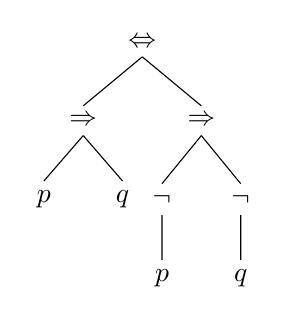
\begin{tikzpicture}[
      level distance=1cm,
      sibling distance=1.5cm,
      level 2/.style={sibling distance=1cm},
      edge from parent path={(\tikzparentnode.south) -- (\tikzchildnode.north)}
    ]
    \node {$\Leftrightarrow$}
      child { 
        node {$\Rightarrow$}
        child { node {$p$} }
        child { node {$q$} }
      }
      child { 
        node {$\Rightarrow$}
        child { node {$\neg$} child { node {$p$} } }
        child { node {$\neg$} child { node {$q$} } }
      };
    \end{tikzpicture}
    }  
  \hfill
  \resizebox{0.35\textwidth}{!}{
    \begin{tikzpicture}[
      level distance=1cm,
      sibling distance=1.5cm,
      level 2/.style={sibling distance=1cm},
      level 3/.style={sibling distance=0.7cm},
      edge from parent path={(\tikzparentnode.south) -- (\tikzchildnode.north)}
    ]
    \node {$\Rightarrow$}
      child { node {$p$} }
      child { 
        node {$\Leftrightarrow$}
        child { node {$q$} }
        child { 
          node {$\neg$}
          child { 
            node {$\Rightarrow$}
            child { node {$p$} }
            child { node {$\neg$} child { node {$q$} } }
          }
        }
      };
    \end{tikzpicture}
    }
  \end{latin}
  \renewcommand{\thefigure}{\lr{2.1}}
  \caption{دو فرمول}
  \end{figure}
  \begin{latin}
  \begin{verbatim}
  Inorder(F):
      if F is a leaf:
          print its label
          return
      Let F1 and F2 be the left and right subtrees of F
      Inorder(F1)
      print the label of the root of F
      Inorder(F2)
  \end{verbatim}
  \end{latin}
  اگر ریشه‌ی $F$ با نماد $\neg$ برچسب‌گذاری شده باشد، زیر‌درخت چپ نادیده گرفته می‌شود و مرحله‌ی \lr{Inorder(F1)} انجام نمی‌گیرد.
  \begin{definition}[تعریف \lr{2.5}]
  اصطلاح «فرمول» برای رشته نیز به‌کار می‌رود، با این فرض که به درخت زیربنایی آن اشاره دارد.
  \end{definition}
  \begin{example}[مثال \lr{2.6}]
  فرمول سمت چپ در شکل \lr{2.1} را در نظر بگیرید. پیمایش درون‌گرد این فرمول به‌صورت زیر است: ابتدا برگ سمت چپ با برچسب $p$ نوشته می‌شود، سپس ریشه‌ی آن که با $\rightarrow$ برچسب‌گذاری شده، سپس برگ سمت راست آن که $q$ است، و سپس ریشه‌ی کل درخت که با $\leftrightarrow$ برچسب‌گذاری شده، و به همین ترتیب ادامه می‌یابد. نتیجه‌ی پیمایش رشته‌ی زیر است:
  \[
  p \rightarrow q \leftrightarrow \neg p \rightarrow \neg q
  \]
  اکنون فرمول سمت راست در شکل \lr{2.1} را در نظر بگیرید. پیمایش آن نیز دقیقاً همین رشته را تولید می‌کند:
  \[
  p \rightarrow q \leftrightarrow \neg p \rightarrow \neg q
  \]
  \end{example}
\subsection*{\lr{2.1.3} رفع ابهام در نمایش رشته‌ای}
   \subsubsection*{پرانتزها}
      
     ساده‌ترین روش برای جلوگیری از ابهام، استفاده از پرانتزها برای حفظ ساختار درخت هنگام تولید رشته است.
      
     \paragraph{الگوریتم \lr{2.7} (نمایش فرمول به‌صورت رشته با پرانتز)} \hfill \\
     \textbf{ورودی:} یک فرمول $A$ از منطق گزاره‌ای \\
     \textbf{خروجی:} نمایش رشته‌ای از $A$ با استفاده از پرانتزها
      
     رویه‌ی بازگشتی زیر را فراخوانی کن: \lr{Inorder(A)}
      
     \begin{latin}
      \begin{verbatim}
      Inorder(F):
          if F is a leaf:
              print its label
              return
          Let F1 and F2 be the left and right subtrees of F
          print '('
          Inorder(F1)
          print the label of the root of F
          Inorder(F2)
          print ')'
      \end{verbatim}
     \end{latin}
   
     اگر ریشه‌ی $F$ با نماد $\neg$ برچسب‌گذاری شده باشد، زیر‌درخت چپ نادیده گرفته می‌شود و مرحله‌ی \lr{Inorder(F1)} انجام نمی‌گیرد.
   
     در این حالت، دو فرمول موجود در شکل \lr{2.1} به دو رشته‌ی متفاوت نگاشته می‌شوند و دیگر ابهامی وجود ندارد:
     \[
     ((p \rightarrow q) \leftrightarrow ((\neg q) \rightarrow (\neg p)))
     \]
     \[
     (p \rightarrow (q \leftrightarrow (\neg (p \rightarrow (\neg q)))))
     \]
   
     مشکل استفاده از پرانتزها آن است که فرمول‌ها را طولانی کرده و خواندن و نوشتن آن‌ها را دشوار می‌سازد.
   
   \subsubsection*{اولویت}
     
     روش دوم برای رفع ابهام در فرمول‌های مبهم، تعریف \textbf{اولویت} (precedence) و \\ \textbf{جهت انجمنی} (associativity) بین عملگرها است، همان‌طور که در حساب معمول انجام می‌شود. برای مثال، عبارت \\ \lr{a * b * c + d * e} بلافاصله به‌صورت \[
     (((a * b) * c) + (d * e))
     \] تفسیر می‌شود.
     
     در مورد فرمول‌های منطقی، ترتیب اولویت از بالا به پایین به‌صورت زیر است:
     
     \[ \\
     \neg \\
     \]
     \[
     \land, \uparrow \\
     \]
     \[
     \lor, \downarrow \\
     \]
     \[
     \rightarrow \\
     \]
     \[
     \leftrightarrow, \oplus
     \]
     عملگرها به‌طور پیش‌فرض \textbf{از راست به چپ} گروه‌بندی می‌شوند (جهت انجاسی راست‌گرا)، یعنی فرمول $a \lor b \lor c$ به‌صورت $a \lor (b \lor c)$ تفسیر می‌شود.
     
     پرانتزها تنها زمانی استفاده می‌شوند که بخواهیم ترتیبی متفاوت از قواعد اولویت و جهت پیش‌فرض را نشان دهیم؛ مانند حساب معمول که در آن \lr{a * (b + c)} به معنای انجام جمع پیش از ضرب است.
     
     با حداقل استفاده از پرانتز، دو فرمول مثال در شکل \lr{2.1} را می‌توان به‌صورت زیر نوشت:
     
     \[
     p \rightarrow q \leftrightarrow \neg q \rightarrow \neg p
     \]
     \[
     p \rightarrow (q \leftrightarrow \neg (p \rightarrow \neg q))
     \]
     
     برای وضوح بیشتر، همیشه می‌توان از پرانتزهای اضافی استفاده کرد؛ مثلاً:
     \[
     (p \lor q) \land (q \lor r)
     \]
     
     عملگرهای بولی $\land$, $\lor$, $\leftrightarrow$, $\oplus$ انجاسی هستند، بنابراین در فرمول‌هایی که شامل تکرار این عملگرها هستند، اغلب پرانتزها حذف می‌شوند؛ مثلاً:
     \[
     p \lor q \lor r \lor s
     \]
     
     اما توجه داشته باشید که عملگرهای $\rightarrow$, $\downarrow$, $\uparrow$ \textbf{غیرانجاسی} هستند، بنابراین استفاده از پرانتز برای جلوگیری از ابهام الزامی است.
     
     اگرچه فرض بر این است که $\rightarrow$ راست‌گرا است و فرمول $p \rightarrow q \rightarrow r$ را به‌صورت $p \rightarrow (q \rightarrow r)$ تفسیر می‌کنیم، اما معمولاً برای وضوح بیشتر، آن را همراه با پرانتز می‌نویسیم:
     \[
     (p \rightarrow q) \rightarrow r
     \]
     
   \subsubsection*{نمادگذاری لهستانی \lr{(Polish Notation)}}
 
    اگر نمایش رشته‌ای یک فرمول با استفاده از پیمایش \textbf{پیش‌گرد} \lr{(preorder traversal)} درخت آن انجام شود، دیگر ابهامی نخواهیم داشت.
 
    \paragraph{الگوریتم \lr{2.8} (نمایش فرمول به‌صورت رشته در نماد لهستانی)} \hfill \\
    \textbf{ورودی:} یک فرمول $A$ از منطق گزاره‌ای \\
    \textbf{خروجی:} نمایش رشته‌ای از $A$ در نمادگذاری لهستانی
 
    رویه‌ی بازگشتی زیر را فراخوانی کن: \lr{Preorder(A)}
 
    \begin{latin}
      \begin{verbatim}
      Preorder(F):
          print the label of the root of F
          if F is a leaf:
              return
          Let F1 and F2 be the left and right subtrees of F
          Preorder(F1)
          Preorder(F2)
      \end{verbatim}
    \end{latin}
 
    اگر ریشه‌ی $F$ با نماد $\neg$ برچسب‌گذاری شده باشد، زیر‌درخت چپ نادیده گرفته می‌شود و مرحله‌ی \lr{Preorder(F1)} انجام نمی‌گیرد.
 
    \begin{example}[مثال \lr{2.9}] رشته‌های مربوط به دو فرمول موجود در شکل \lr{2.1} در نمادگذاری لهستانی به‌صورت زیر هستند:
      \[
      \leftrightarrow\ \rightarrow\ p\ q\ \rightarrow\ \neg p\ \neg q
      \]
      \[
      \rightarrow\ p\ \leftrightarrow\ q\ \neg\ \rightarrow\ p\ \neg q
      \]
    و اکنون دیگر هیچ ابهامی وجود ندارد.
    \end{example}
    فرمول‌هایی که به این صورت نمایش داده می‌شوند، گفته می‌شود در \textbf{نمادگذاری لهستانی} هستند، که به افتخار گروهی از منطق‌دانان لهستانی به رهبری \lr{Jan Łukasiewicz} نام‌گذاری شده است.
 
    ما نمایش درون‌گرد (\lr{infix}) را خواناتر می‌دانیم، چراکه در حساب معمول نیز رایج است. بنابراین نمادگذاری لهستانی معمولاً تنها برای نمایش درونی عبارات حسابی و منطقی در رایانه‌ها استفاده می‌شود. مزیت اصلی آن این است که می‌توان فرمول را در همان ترتیبی که نمادها ظاهر می‌شوند با استفاده از یک \lr{stack} ارزیابی کرد.
 
    اگر فرمول اول را به‌صورت معکوس بازنویسی کنیم (که به آن \textbf{نمادگذاری لهستانی معکوس} یا \lr{RPN} نیز گفته می‌شود):
 
    \[
    q\ \neg\ p\ \neg\ \rightarrow\ q\ p\ \rightarrow\ \leftrightarrow
    \]
 
    می‌توان آن را مستقیماً به دنباله‌ای از دستورات اسمبلی زیر ترجمه کرد:
 
    \begin{latin}
      \begin{verbatim}
      Push q
      Negate
      Push p
      Negate
      Imply
      Push q
      Push p
      Imply
      Equiv
      \end{verbatim}
    \end{latin}
 
    در این روش، عملگرها روی عملوندهایی که در بالای پشته قرار دارند اعمال می‌شوند، سپس عملوندها از پشته خارج (pop) شده و نتیجه روی پشته قرار داده می‌شود.
\subsection*{\lr{2.1.4} \quad استقرا ساختاری}
 
  اگر یک عبارت حسابی مانند \lr{a * b + b * c} را در نظر بگیریم، به‌راحتی می‌توان دید که این عبارت از دو جمله تشکیل شده که با عملگر جمع ترکیب شده‌اند، و هر جمله‌ی جمعی نیز از دو عامل ضرب تشکیل شده است. به‌طور مشابه، هر فرمول گزاره‌ای را می‌توان بر اساس عملگر سطح بالای آن طبقه‌بندی کرد.
 
  \begin{definition}[تعریف \lr{2.10}]
    اگر $A \in \mathscr{F}$ و $A$ یک اتم نباشد، عملگری که ریشه‌ی درخت فرمول $A$ را برچسب‌گذاری می‌کند، \textbf{عملگر اصلی} (\lr{principal operator}) فرمول $A$ نامیده می‌شود.
  \end{definition}
  \begin{example}[مثال \lr{2.11}]
    عملگر اصلی فرمول سمت چپ در شکل \lr{2.1}، عملگر $\leftrightarrow$ و در فرمول سمت راست، عملگر $\rightarrow$ است.\\
  \end{example}

  استقرا ساختاری روشی برای اثبات این است که یک خاصیت برای همه‌ی فرمول‌ها برقرار است. این شکل از استقرا، مشابه \textbf{استقرای عددی} آشنایی است که برای اثبات خاصیت برای همه‌ی اعداد طبیعی به‌کار می‌رود (بخش \lr{A.6} را ببینید). در استقرای عددی:

  \begin{itemize}
    \item \textbf{گام پایه:} اثبات خاصیت برای صفر است، و
    \item \textbf{گام استقرا:} فرض می‌کنیم خاصیت برای عدد دلخواه $n$ برقرار است و سپس اثبات می‌کنیم که برای $n+1$ نیز برقرار خواهد بود.
  \end{itemize}

  بر اساس تعریف \lr{2.10}، یک فرمول یا:
  \begin{itemize}
    \item یک برگ با برچسب اتم است،
    \item یا یک درخت با عملگر اصلی و یک یا دو زیر‌درخت.
  \end{itemize}

  بنابراین، در استقرا ساختاری:
  \begin{itemize}
    \item \textbf{گام پایه:} اثبات خاصیت برای برگ‌ها (اتم‌ها) است.
    \item \textbf{گام استقرا:} اثبات خاصیت برای فرمولی است که از به‌کارگیری عملگر اصلی روی زیر‌فرمول‌ها به‌دست آمده، مشروط بر آنکه خاصیت برای آن زیر‌فرمول‌ها برقرار باشد.
  \end{itemize}

  \begin{theorem}[قضیه \lr{2.12} (استقرا ساختاری). ]
   برای اینکه نشان دهیم خاصیتی برای همه‌ی فرمول‌ها $A \in \mathscr{F}$ برقرار است، کافی است:
   
   \begin{enumerate}
     \item اثبات کنیم که خاصیت برای تمام اتم‌ها $p$ برقرار است.
     \item فرض کنیم خاصیت برای فرمولی مانند $A$ برقرار است و اثبات کنیم که خاصیت برای $\neg A$ نیز برقرار است.
     \item فرض کنیم خاصیت برای فرمول‌های $A_1$ و $A_2$ برقرار است، و اثبات کنیم که خاصیت برای $A_1 \mathbin{\operatorname{op}} A_2$ نیز برقرار است، برای هر یک از عملگرهای دوجمله‌ای.
   \end{enumerate}
  \end{theorem}

  \begin{proof}[اثبات. ]
    فرض کنیم $A$ یک فرمول دلخواه باشد و فرض کنیم که بندهای (۱)، (۲)، (۳) برای خاصیت مورد نظر اثبات شده‌اند. ما نشان می‌دهیم که خاصیت برای $A$ برقرار است، با استفاده از استقرای عددی بر حسب $n$، که ارتفاع درخت مربوط به $A$ است:
    \begin{itemize}
      \item اگر $n = 0$ باشد، درخت یک برگ است، بنابراین $A$ یک اتم $p$ است و خاصیت طبق بند (۱) برقرار است.
      \item اگر $n > 0$ باشد، زیر‌درخت‌های $A$ ارتفاعی برابر با $n - 1$ دارند، بنابراین طبق فرض استقرای عددی، خاصیت برای آن‌ها برقرار است. از آنجا که عملگر اصلی $A$ یا نقیض ($\neg$) است یا یکی از عملگرهای دوجمله‌ای، بنابراین طبق بند (۲) یا (۳)، خاصیت برای $A$ نیز برقرار است.
    \end{itemize}
  \end{proof}
  بعداً نشان خواهیم داد که تمام عملگرهای دوجمله‌ای را می‌توان با ترکیب نقیض و یکی از دو عملگر $\lor$ یا $\land$ تعریف کرد؛ بنابراین، برای اثبات خاصیت برای همه‌ی فرمول‌ها، کافی است از استقرا ساختاری با حالت پایه و تنها دو گام استقرا استفاده کنیم.
\subsection*{\lr{2.1.5} \quad نمادگذاری}
  متأسفانه، در کتاب‌های مختلف منطق ریاضی، نمادهای مورد استفاده برای عملگرهای بولی یکسان نیستند؛ افزون بر این، در زبان‌های برنامه‌نویسی نیز این عملگرها معمولاً با نمادهایی متفاوت از آنچه در منابع ریاضی دیده می‌شود نمایش داده می‌شوند. جدول زیر، برخی از این نمادهای جایگزین را نشان می‌دهد:
  \begin{center}
    \begin{tabular}{|c|c|c|}
    \hline
    \textbf{عملگر} & \textbf{نمادهای جایگزین} & \textbf{زبان \lr{Java}} \\
    \hline
    $\neg$ & \lr{\textasciitilde} & \lr{!} \\
    \hline
    $\land$ & \lr{\&} & \lr{\&}, \lr{\&\&} \\
    \hline
    $\lor$ &  & \lr{|}, \lr{||} \\
    \hline
    $\rightarrow$ & $\supset$, $\Rightarrow$ & \\
    \hline
    $\leftrightarrow$ & $\equiv$, $\Leftrightarrow$ & \\
    \hline
    $\oplus$ & $\not\equiv$ & \lr{\^{}} \\
    \hline
    $\uparrow$ & \lr{|} &  \\
    \hline
    \end{tabular}
  \end{center}
\subsection*{\lr{2.1.6} \quad دستور زبان صوری برای فرمول ها}
  (این زیر‌بخش مستلزم آشنایی با دستور زبان‌های صوری است.)
  به‌جای تعریف فرمول‌ها به‌صورت درختی، می‌توان آن‌ها را به‌شکل رشته‌هایی تعریف کرد که از یک دستور زبان مستقل از متن (\lr{context-free grammar}) تولید می‌شوند.
  \begin{definition}[تعریف \lr{2.13}]
    فرمول‌های منطق گزاره‌ای از دستور زبانی مستقل از متن تولید می‌شوند که نمادهای پایانی (\lr{terminal symbols}) آن به‌صورت زیر تعریف شده‌اند:
    \begin{itemize}
      \item مجموعه‌ای نامتناهی از نمادها به‌نام گزاره‌های اتمی \lr{$\mathcal{P}$}
      \item عملگرهای بولی مطابق با تعریف \lr{2.1}
    \end{itemize}
    قواعد تولید (\lr{production rules}) این دستور زبان به‌صورت زیر هستند:
    \begin{align*}
      \text{fml} &::= p \qquad \text{برای هر } p \in \mathcal{P} \\
      \text{fml} &::= \neg \text{ fml} \\
      \text{fml} &::= \text{fml op fml} \\
      \text{op} &::= \lor \mid \land \mid \rightarrow \mid \leftrightarrow \mid \oplus \mid \uparrow \mid \downarrow
    \end{align*}
    یک فرمول، رشته‌ای است که می‌توان آن را از نماد غیرپایانی \lr{fml} استخراج کرد. مجموعه‌ی تمام فرمول‌هایی که از این دستور زبان به‌دست می‌آیند با نماد $\mathscr{F}$ نمایش داده می‌شود.
    فرآیند تولید (اشتقاق) رشته‌ها در یک دستور زبان صوری را می‌توان با درخت‌های اشتقاق \\ (\lr{derivation trees}) نمایش داد . رشته‌ی نهایی را می‌توان از طریق خواندن برگ‌ها از چپ به راست به‌دست آورد.
  \end{definition}
  \begin{example}[مثال \lr{2.14}]
    در ادامه، فرآیند اشتقاق فرمول زیر در منطق گزاره‌ای نشان داده شده است:
    \[
    p \rightarrow q \leftrightarrow \neg p \rightarrow \neg q
    \]
    \begin{figure}[ht]
    \centering
    \begin{latin}
    \resizebox{0.7\textwidth}{!}{%
    \begin{tikzpicture}[
      level distance=1.5cm,
      sibling distance=4cm,
      level 2/.style={sibling distance=2cm},
      level 3/.style={sibling distance=1cm},
      edge from parent path={(\tikzparentnode.south) -- (\tikzchildnode.north)}
    ]
    \node {fml}
      child { 
        node {fml}
        child { 
        	node {fml}
        	child {node {$p$}}
        }
        child {
        	node {op}
        	child {node {$\Rightarrow$}}
        }
        child { 
        	node {fml} 
        	child {node {$q$}}
        }
      }
      child { 
        node {op}
        child {node {$\Leftrightarrow$}}
        child { 
          node {fml}
          child { 
            node {fml}
            child {node {$\neg$}}
            child {node {fml}
              child {node {$p$}}
            }
          }
          child {
            node {op}
            child {node {$\Rightarrow$}}
          }
          child { 
            node {fml}
            child {node {$\neg$}}
            child {node {fml}
              child {node {$q$}}
            }
          }
        }
      };
    \end{tikzpicture}
    }
    \end{latin}
    \renewcommand{\thefigure}{\lr{2.2}}
    \caption{اشتقاق درخت برای $p \rightarrow q \leftrightarrow \neg p \rightarrow \neg q$ }
    \end{figure}
    درخت مربوطه در شکل \lr{2.2} آمده است. گام‌های اشتقاق به‌صورت زیر هستند:
    \begin{align*}
      1.\quad & \text{fml} \\
      2.\quad & \text{fml op fml} \\
      3.\quad & \text{fml} \leftrightarrow \text{fml} \\
      4.\quad & \text{fml} \rightarrow \text{fml} \leftrightarrow \text{fml} \\
      5.\quad & p \rightarrow \text{fml} \leftrightarrow \text{fml} \\
      6.\quad & p \rightarrow q \leftrightarrow \text{fml} \\
      7.\quad & p \rightarrow q \leftrightarrow \text{fml} \rightarrow \text{fml} \\
      8.\quad & p \rightarrow q \leftrightarrow \neg \text{fml} \rightarrow \text{fml} \\
      9.\quad & p \rightarrow q \leftrightarrow \neg p \rightarrow \text{fml} \\
      10.\quad & p \rightarrow q \leftrightarrow \neg p \rightarrow \neg \text{fml} \\
      11.\quad & p \rightarrow q \leftrightarrow \neg p \rightarrow \neg q
    \end{align*}
  \end{example}
  روش‌هایی که در بخش \lr{2.1.2} برای رفع ابهام معرفی شدند، در اینجا نیز قابل‌استفاده هستند.
  همچنین می‌توان دستور زبان را طوری بازنویسی کرد که پرانتزها را به‌صورت درونی دربر گیرد:
  \begin{align*}
    \text{fml} &::= (\neg \text{fml}) \\
    \text{fml} &::= (\text{fml op fml})
  \end{align*}
  و سپس با تعریف قواعد اولویت، می‌توان تعداد پرانتزها را کاهش داد.
  
  \begin{figure}[ht]
  \centering
    \begin{RTL}
      \begin{tabbing}
      \hspace{6.5cm} \= \kill
        $v_{\mathscr{I}}(A) = \mathscr{I}_A(A)$ \> اگر $A$ یک اتم باشد \\
        $v_{\mathscr{I}}(\neg A) = T$ \> اگر $v_{\mathscr{I}}(A) = F$ \\
        $v_{\mathscr{I}}(\neg A) = F$ \> اگر $v_{\mathscr{I}}(A) = T$ \\
        $v_{\mathscr{I}}(A_1 \lor A_2) = F$ \> اگر $v_{\mathscr{I}}(A_1) = F$ و $v_{\mathscr{I}}(A_2) = F$ \\
        $v_{\mathscr{I}}(A_1 \lor A_2) = T$ \> در غیر این صورت \\
        $v_{\mathscr{I}}(A_1 \land A_2) = T$ \> اگر $v_{\mathscr{I}}(A_1) = T$ و $v_{\mathscr{I}}(A_2) = T$ \\
        $v_{\mathscr{I}}(A_1 \land A_2) = F$ \> در غیر این صورت \\
        $v_{\mathscr{I}}(A_1 \rightarrow A_2) = F$ \> اگر $v_{\mathscr{I}}(A_1) = T$ و $v_{\mathscr{I}}(A_2) = F$ \\
        $v_{\mathscr{I}}(A_1 \rightarrow A_2) = T$ \> در غیر این صورت \\
        $v_{\mathscr{I}}(A_1 \uparrow A_2) = F$ \> اگر $v_{\mathscr{I}}(A_1) = T$ و $v_{\mathscr{I}}(A_2) = T$ \\
        $v_{\mathscr{I}}(A_1 \uparrow A_2) = T$ \> در غیر این صورت \\
        $v_{\mathscr{I}}(A_1 \downarrow A_2) = T$ \> اگر $v_{\mathscr{I}}(A_1) = F$ و $v_{\mathscr{I}}(A_2) = F$ \\
        $v_{\mathscr{I}}(A_1 \downarrow A_2) = F$ \> در غیر این صورت \\
        $v_{\mathscr{I}}(A_1 \leftrightarrow A_2) = T$ \> اگر $v_{\mathscr{I}}(A_1) = v_{\mathscr{I}}(A_2)$ \\
        $v_{\mathscr{I}}(A_1 \leftrightarrow A_2) = F$ \> اگر $v_{\mathscr{I}}(A_1) \ne v_{\mathscr{I}}(A_2)$ \\
        $v_{\mathscr{I}}(A_1 \oplus A_2) = T$ \> اگر $v_{\mathscr{I}}(A_1) \ne v_{\mathscr{I}}(A_2)$ \\
        $v_{\mathscr{I}}(A_1 \oplus A_2) = F$ \> اگر $v_{\mathscr{I}}(A_1) = v_{\mathscr{I}}(A_2)$ \\
      \end{tabbing}
    \end{RTL}
    \renewcommand{\thefigure}{\lr{2.3}}
    \caption{مقادیر منطقی فرمول‌ها}
  \end{figure}